\chapter{Introduction}

\begin{enumerate}
    \item Motivation \& Relevance
    \item Domain and Motivation: e.g. \ac{SAR}, semantic Navigation, exploration in unknown environments, etc.
    \item Which solutions exist? Comparison of general properties and performance metrics:
    \begin{enumerate}
        \item \ac{OneMap} \cite{busch2025onemap}
        \item \ac{VLMaps} \cite{huang23vlmaps}
        \item \ac{VLFM} \cite{yokoyama2024vlfm}
        \item \ac{ConceptGraphs} \cite{gu2023conceptgraphsopenvocabulary3dscene}
        \item \ac{SemExp} \cite{chaplot2020semexp}
        \item \ac{GeFF} \cite{qui2024geff}
    \end{enumerate}

    \begin{figure}[h!]
    \centering
    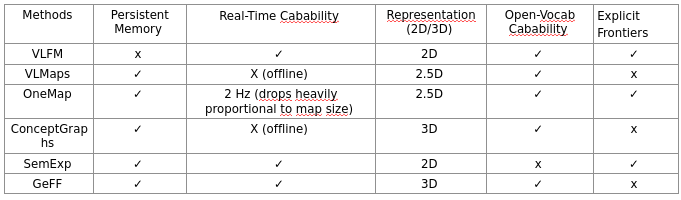
\includegraphics[width=\textwidth]{Images/1_introduction/temp_sota_comparison_common_properties.png}
    \caption{Comparison of state-of-the-art methods regarding common properties.}
    \label{fig:sota_comparison}
    \end{figure}

    \begin{figure}[h!]
    \centering
    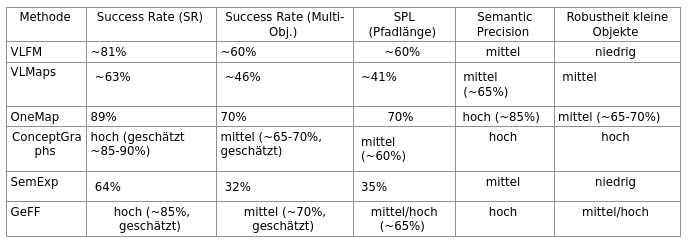
\includegraphics[width=\textwidth]{Images/1_introduction/temp_sota_comparison_performance_metrics.png}
    \caption{Comparison of state-of-the-art methods regarding performance metrics.}
    \label{fig:sota_performance}
    \end{figure}

    \item What is the technical problem? A combination of the following:
    \begin{enumerate}
        \item No persistent memory
        \item Not Real-Time
        \item 3D-Representation
        \item Sensibility to false positives for zero shot object detection
    \end{enumerate}
    \item Scientific Contribution:
    \begin{itemize}
        \item Development of a hybrid approach that combines \ac{VLFM} \cite{yokoyama2024vlfm} and Open-Fusion \cite{kashu2023openfusion} to increase overall \ac{SR} and specifically enhance multi-object \ac{SR} compared to state-of-the-art methods such as \ac{OneMap}, \ac{VLMaps}, and \ac{GeFF}.
        \item Investigation of whether integrating fast frontier exploration (\ac{VLFM}) with explicitly segmented nodes (Open-Fusion) enables shorter and more efficient navigation paths, leading to improved path efficiency measured by the \ac{SPL} metric.
        \item Design of a sensor-based fusion strategy leveraging spatially weighted score combination, where \ac{SEEM} \cite{zou2023seem} detections and OpenFusion \cite{kashu2023openfusion} relevance fields are merged using Gaussian-based weighting to increase robustness against false positives in zero-shot detection scenarios.
        \item Evaluation of the proposed method’s performance in real-world scenarios on a mobile robot, focusing on practical aspects such as real-time capability and robustness to sensor noise, including depth inaccuracies and varying lighting conditions.
    \end{itemize}
    \item Structure of the thesis:
\end{enumerate}
